%%%%%%%%%%%%%%%%%%%%%%%%%%%%%%%%%%%%%%%%%
% University/School Laboratory Report
% LaTeX Template
% Version 3.1 (25/3/14)
%
% This template has been downloaded from:
% http://www.LaTeXTemplates.com
%
% Original author:
% Linux and Unix Users Group at Virginia Tech Wiki 
% (https://vtluug.org/wiki/Example_LaTeX_chem_lab_report)
%
% License:
% CC BY-NC-SA 3.0 (http://creativecommons.org/licenses/by-nc-sa/3.0/)
%
%%%%%%%%%%%%%%%%%%%%%%%%%%%%%%%%%%%%%%%%%

%----------------------------------------------------------------------------------------
%	PACKAGES AND DOCUMENT CONFIGURATIONS
%----------------------------------------------------------------------------------------

\documentclass[paper=a4, fontsize=11pt]{scrartcl} % A4 paper and 11pt font size

\usepackage[version=3]{mhchem} % Package for chemical equation typesetting
\usepackage{siunitx} % Provides the \SI{}{} and \si{} command for typesetting SI units
\usepackage{graphicx} % Required for the inclusion of images
%\usepackage{natbib} % Required to change bibliography style to APA
\usepackage{amsmath} % Required for some math elements 
\usepackage{wrapfig}
\usepackage{url}
\usepackage{hyperref}


\setlength\parindent{0pt} % Removes all indentation from paragraphs

\renewcommand{\labelenumi}{\alph{enumi}.} % Make numbering in the enumerate environment by letter rather than number (e.g. section 6)

%\usepackage{times} % Uncomment to use the Times New Roman font

%----------------------------------------------------------------------------------------
%	DOCUMENT INFORMATION
%----------------------------------------------------------------------------------------

\title{Project 2 \\ SQuAD machine comprehension report \\ CS5242} % Title

\author{Group 16} % Author name

\date{\today} % Date for the report

\begin{document}

\maketitle % Insert the title, author and date

\begin{center}
\begin{tabular}{l r}
%Date Performed: & January 1, 2012 \\ % Date the experiment was performed
Partners: & Kyaw Zaw Lin(E0218306) \\ % Partner names
& Luu Tuan Nghia(E0013431) \\

\end{tabular}
\end{center}

% If you wish to include an abstract, uncomment the lines below
% \begin{abstract}
% Abstract text
% \end{abstract}

%----------------------------------------------------------------------------------------
%	SECTION 1
%----------------------------------------------------------------------------------------

\section{Problem definition}
%\setlength{\columnsep}{10pt}%
%\setlength{\intextsep}{10pt}%
\begin{wrapfigure}{r}{0.3\textwidth}\centering
	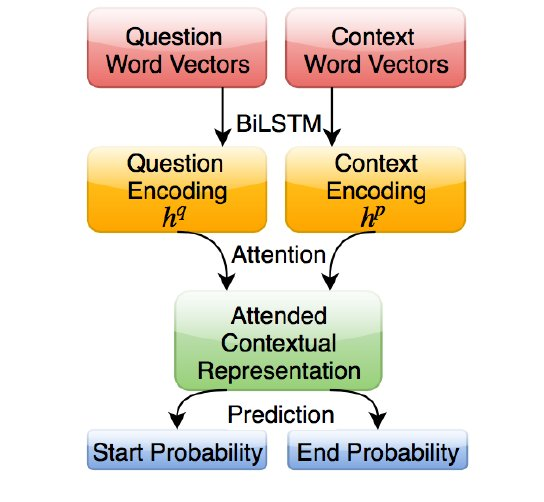
\includegraphics[scale=0.2]{gen_model.jpg}
	\caption{General model for QA tasks}
	\label{fig:gen_model}
\end{wrapfigure}
%\setlength{\intextsep}{0pt}%

Reading texts and answering questions are common tasks in NLP. In this project, we developed a model that is able to answer questions automatically given an associated context paragraph. 
With the developed model, each answer is a set of consecutive words from the original context paragraph. The model architecture allows it to work with any language, however, because word vectors are processed using an English dictionary, the model will only work with English language for now.

Based on literature review,the majority of state-of-the-art works follow this general design shown in Fig \ref{fig:gen_model}, where questions and context are separately represented by different embeddings and the model output start and end probability.

\section{Models investigated}
The model we developed is the combination of 3 different models: Bidirectional Attention Flow(BiDAF) \cite{DBLP:journals/corr/SeoKFH16}, DrQA\cite{DBLP:journals/corr/ChenFWB17} and Simple Recurrent Unit(SRU) \cite{DBLP:journals/corr/abs-1709-02755}. All 3 models were trained separately so that they can handle question answering tasks independently. The results of all 3 models were then combined by voting with some weights. The weights were chosen so that the models with higher accuracy when testing alone would have higher weights. The intuition was to trust better models more.
The details of individual model architectures are explained below.

\subsection{BiDAF}
The model is based on LSTM, its architecture is shown in Fig \ref{fig:bidaf}.
\begin{figure}[!htb]\centering
	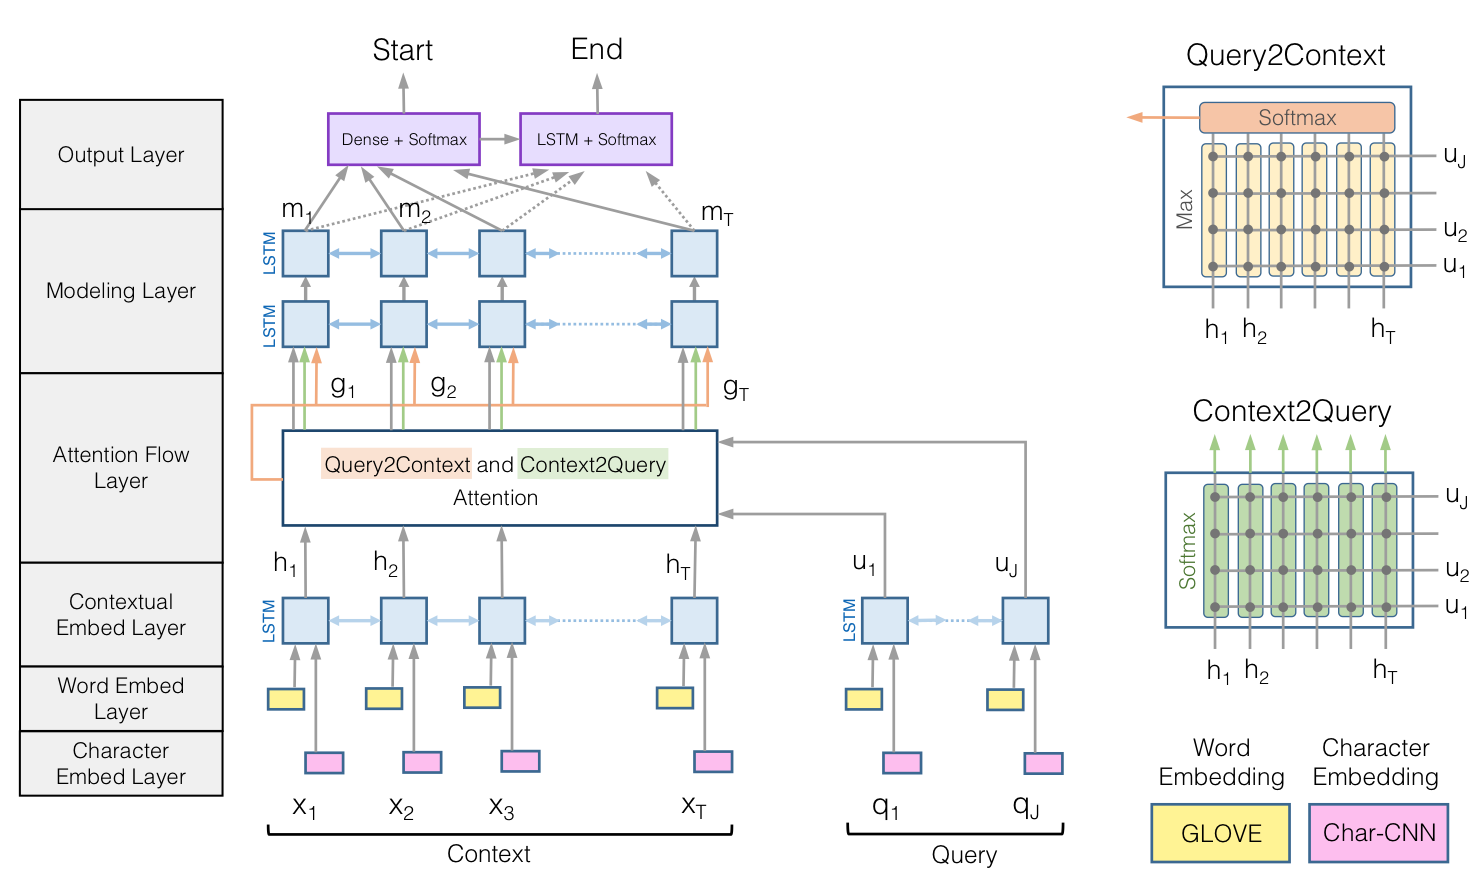
\includegraphics[scale=0.5]{bidaf.png}
	\caption{BiDAF Framework}
	\label{fig:bidaf}
\end{figure}
The architecture consists of 6 layers:
\begin{itemize}
	\item Character embedding layer: this layer embeds words into high dimensional vectors using character-level CNNs.
	\item Word-embedding layer: maps words into high dimensional vectors using GloVe (pre-trained word embedding model).
	\item Contextual layer: Using LSTMs in both directions to capture temporal relationship between words.
	\item Attention flow layer: combine context and query vectors and produce a set of query-aware vectors.
	\item Modelling layer: Using LSTMs to scan the context from the output of attention flow layer.
	\item Output layer: provides an answer for the query.
\end{itemize}

\subsection{DrQA}
DrQA is a system designed to answer open domain questions by using Wikipedia corpus. The system is composed of Document Retriever, which is a classical information retrieval module and the Document Reader, which is the machine comprehension component used on the rough results of Document Retriever. Document Reader is trained on SQuAD and is generally similar in overall design with bi-att-flow with the following differences:
\begin{itemize}
	\item Paragraph encoding: Each paragraph is encoded by a multi-layer bidirectional LSTM into vectors which represent the main context of the paragraph. In order to do so, DrQA uses the following features:
	\begin{itemize}
		\item Embedded words: words are embedded using GloVe into 300-dimensional vectors. 
		\item Exact match: indicating whether a paragraph matches exactly with a question word.
		\item Token features: embed useful information such as term frequency.
		\item Aligned question embedding: similar to exact match, it specifies the similarity between a paragraph and a question.
	\end{itemize}
	\item Question encoding: Embed each question into a vector using a simple LSTM with embed words from the question.
\end{itemize}

After encoding paragraphs and questions, Document Reader predicts the span of the answer for each question by calculating the probability of start index and end index of the answer. 

\subsection{Simple Recurrent Unit (SRU)}
SRU is a technique to improve the speed of RNNs. Typical RNNs which use LSTMs to compete with gradient vanishing/exploding over a long distance usually take a long time to train. The reason is that each network layer depends on the output of the previous layer. Therefore the layers cannot be calculated in parallel.
SRU overcomes this issue by making the gate computation depend only on the current layer’s input. The results of all layers are combined via a fast recurrent structure. The difference between SRU models and LTSM models is shown in Fig \ref{fig:sru}.
In our project, we used a model of DrQA which made use of SRU technique in hope of speeding up the training. This model performs slightly better than DrQA due to different set of hyperparameters.
\begin{figure}[htb]\centering
	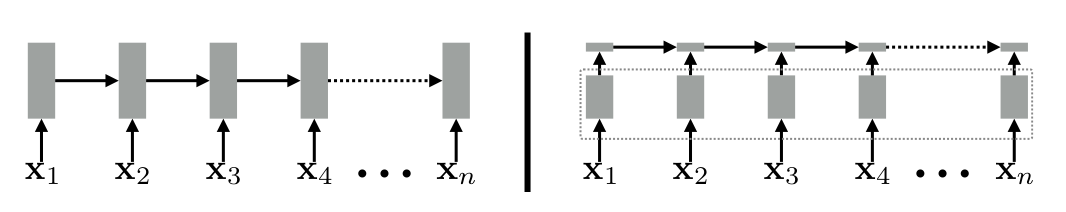
\includegraphics[scale=0.5]{sru.png}
	\caption{LSTM architecture is shown on the left, and SRU architecture is shown on the right.}
	\label{fig:sru}
\end{figure}

\section{Ensembling}
Our ensembling strategy is a simple weighted voting requiring only the csv file uploaded to kaggle. It can be described as follow:

\begin{align} 
\begin{split}
y = \underset{a_i \in A }{\operatorname{arg\,max}} \sum_{j = 1}^m w_jX_A(M_j(x)=a_i)	 
\end{split}					
\end{align} 

where the indicator function $X_A(M_j(x)=a_i)$ equals $1$ when $M_j(x)=a_i$ and $0$ otherwise. $A$ is the set of all answers and $w_j$ is the weight associated with model $j$. We have considered using probability directly to perform soft weighting. However, we abandon the idea as we are unsure how to calibrate the probabilities from different models.

The weights are first initialized as accuracy on validation set and then were slightly tweaked by submission against Kaggle test platform. In our final submission, we used 6 models, two from each primary models(BiDAF,DrQA,DrQA+SRU). Interestingly, even though BiDAF performs worst, without it the ensemble fails to obtain the best performance. This is likely to do the fact that DrQA and DrQA+SRU share much in common and produce highly correlated answers. Thus low correlated predictions from BiDAF can increase the final performance.


\section{Dataset pre-processing description}
The projects used NUS dataset, which was a subset of the Stanford Question Answering Dataset (SQuAD). The dataset consists of 295 context paragraphs, each with a set of questions. In order to use the dataset efficiently, every word has to be embedded into a word vector so that the distance between 2 word vectors can represent the relationship between 2 words. Uncommon words were not considered as there was too little information about them to make a good use of them. Common words are embedded by using GLoVe (Global Vectors for Word Representation) and Character level CNN. Additional features such as pos tags, named entity and term frequency are used in DrQA.

We have additionally split train dataset with 80:20 ratio into train and validation sets to perform hyperparameter tuning and model selection. The final models are retrained on full set once the optimal parameters are finalized.

\section{Experiments}
The training process was done on 2 machines with 2 TitanX and 2 P40 gpus. Each model was trained separately. It took about 15-20 hours to complete training a model. Different hyperparameters were used during the training process in order to find out the optimum parameters. The parameters which were tried during the training process and their effects are as follow:

\begin{itemize}
	\item Batch size[larger sizes almost always give better performance]
	\item Dropout rate[between .2 and .5 is the best]	
	\item Weight decay[always decrease performance, perhaps due to weights being shared across time, maybe we need to try much smaller weight decays than typical cnn]
	\item Number of layers[almost no effect]
	\item Hidden layer size[larger size slightly increase performance <.5\%]
	\item Different rnn types(rnn,gru,lstm)[lstm performs best]
\end{itemize}

Final performance of each model and combined ensemble is given in Table \ref{tab:results}.

\begin{table}	\centering

	\caption{Performance of different models based on public leaderboard}	\label{tab:results}
	\begin{tabular}{l*{6}{c}r}
		Model              & EM   \\
		\hline
		BiDAF & .5440  \\
		DrQA            & .5848  \\
		DrQA+SRU           & .5934	  \\
		Ensemble(6 models)     & 	.6177  \\

	\end{tabular}

\end{table}

\section{Reflection And Findings}
We first tackled this problem by starting with publically available SQuAD leaderboard and reviewing the related literature of top performers. We adopted the stance that given the amount of research and effort devoted to this topic, and the difficulties researchers have faced in reproducing rnet \footnote{\url{https://yerevann.github.io/2017/08/25/challenges-of-reproducing-r-net-neural-network-using-keras/}}, we feel it is unwise to start coding from scratch and instead opted to use openly available implementations. Our approach can be thought of as a literature review + hyperparameter exploration exercise. 

The first issue we found the importance of batch size, initially we trained on small gpus due to limited memory. However, we are unable to reach the reported accuracies. After we have procured access to large ram gpus, we restarted training with large batch sizes and improvements of 6-7\% can be observed. We believe this is due to the diverse nature of SQuAD dataset and larger batch sizes help smooth out rugged decision boundaries and subsequently improve generalization.

Secondly, we would like to understand the underlying reason for the performance differences between three primary models we have tested. However, due to the large number of differences between the implementation of BiDAF and DrQA, a systematic comparison is not possible. The main differences are:
\begin{itemize}
	\item Different GloVE vector sizes(100 vs 300)
	\item Different nlp preprocessing routines(BiDAF uses nltk/standford and DrQA uses spacy)
	\item Different models
	
\end{itemize}

Post competition, we have performed further experiments by replacing BiDAF original 100d glove vectors with 300d version and observed about 1\% increase in performance. Given that the actual modelling of both implementations follow the overall general design, we think that the difference of 3\% should be due to the manually engineered features that drqa have added. This shows that despite the power of deep learning models, they are still inadequate to fully represent the full range machine understanding of text and still requires manually adjusted features to help.

We have also noticed the problem that longer answers tend to be wrong. Although we did not have time to further explore this, we did a small experiment by choosing the shortest answer of all the models. Unfortunately, this significantly decreases performance. If we continue to work on this project, investigating this issue can be resolved will be our future work.

\bibliographystyle{ieeetr}

\bibliography{report} 

%----------------------------------------------------------------------------------------


\end{document}